\documentclass{article}
\usepackage[utf8]{inputenc}
\usepackage{listings}
\title{CO321 User Manual}
\date{June 2018}
\usepackage{tikz}
\usepackage{pdfpages}

\begin{document}
\begin{titlepage} % Suppresses headers and footers on the title page

	\centering % Centre everything on the title page
	
	\scshape % Use small caps for all text on the title page
	
	\vspace*{\baselineskip} % White space at the top of the page
	
	%------------------------------------------------
	%	Title
	%------------------------------------------------
	
	\rule{\textwidth}{1.6pt}\vspace*{-\baselineskip}\vspace*{2pt} % Thick horizontal rule
	\rule{\textwidth}{0.4pt} % Thin horizontal rule
	
	\vspace{1.5\baselineskip} % Whitespace above the title
	
	{\LARGE NON INVASIVE \\\vspace{5.0pt}INFANT SLEEP APNEA DETECTION \\ \vspace{15.0pt} USER MANUAL} % Title
	
	\vspace{1.5\baselineskip} % Whitespace below the title
	
	\rule{\textwidth}{0.4pt}\vspace*{-\baselineskip}\vspace{3.2pt} % Thin horizontal rule
	\rule{\textwidth}{1.6pt} % Thick horizontal rule
	
	\vspace{2cm} % Whitespace after the title block
	
	%------------------------------------------------
	%	Subtitle
	%------------------------------------------------
	
	CO321 CO324 CO325 Unified Project % Subtitle or further description
	
	\vspace*{6cm} % Whitespace under the subtitle
	
	%------------------------------------------------
	%	Editor(s)
	%------------------------------------------------
	
	Team
	
	\vspace{0.5\baselineskip} % Whitespace before the editors
	
	{\scshape\Large \begin{tabular}{c l}
	     E/14/158: &Gihan Jayatilaka\\E/14/339: &Suren Sritharan\\E/14/379:& Harshana Weligampola\\E/14/237: &Pankayaraj Pathmanathan\\
	\end{tabular} } % Editor list
	
	\vspace{0.5\baselineskip} % Whitespace below the editor list
	
	\textit{Deaprtment of Computer Engineering \\ Unviersity of Peradeniya} % Editor affiliation
	
	\vfill % Whitespace between editor names and publisher logo
	
	%------------------------------------------------
	%	Publisher
	%------------------------------------------------
	
	
	\vspace{0.3\baselineskip} % Whitespace under the publisher logo
	
	2018 % Publication year
	
\end{titlepage}

\tableofcontents
\listoffigures
\clearpage
\section{Introduction}
\subsection{Sleep apnea}
Sleep Apnea is a serious disorder caused by the interruption of breathing during sleep. This can cause the people to stop breathing for several times (even hundreds) if not treated properly. It can affect people of any age. But when the babies are affected with the condition they tend to not get up and keep on sleeping which may risk their lives.

\subsection{The system}
This is a non invasive solution based on video processing. The infant is observed by a video camera which is connected to a single board computer (Raspberry pi) which analyzes the video feed to diagnose breathing anomalies. The camera is turned to a proper orientation for the observation using a robotic arm.

\subsection{Process overview}
The system uses a high definition camera to monitor the baby and a powerful single board computer to process the video to identify the breathing pattern and asses it for anomalies in order to detect \textbf{sleep apnea} using intelligent algorithms. The unit communicates with the web server over the internet which provides an user friendly interface for the doctors and parents to see the reports. 


\section{Features}

\begin{itemize}
    \item Measurement and storage of breathing pattern
    \item Real time alerts
    \item Our solution is $100\%$ non intrusive.
    \item The camera node could operate independently with the inbuilt battery cells. There is no need even for internet connection for the primary functionality.
    \item Our camera can automatically detect the baby and orient itself to the correct position intelligently using the robotic arm.
    \item The \textit{breathing detection algorithm} is automated than the previous work found. (The existing algorithms require human intervention to detect interesting regions etc:)
    \item The \textit{breathing detection algorithm} is accuracte than the existing algorithms.


\end{itemize}

\section{Quick Start up}    %  HARSHANA

This section explains quicker way to test the main functionality of the system.

\begin{enumerate}

  \item Website 
    \begin{enumerate}
      \item Go to http://isad.teambitecode.com/
      \item Signup
      \item Login
      \item Register the device.
    \end{enumerate}

  \item Device
    \begin{enumerate}
      \item Connect to device
      \item Open config.ini file.
      \item Specify user name, device id and access token (Same as registered device).
      \item Press reset button
    \end{enumerate}
    
Now the status LED must become stable after some time. If you press the analyze button next to the device in the device list menu you must be able to observe the graph being plotted.
  
\end{enumerate}


\section{Device Installation}
\begin{itemize}
    \item Connect the device to the computer LAN
    \item Use a \textbf{SSH client} to connect to the node
    \item Enter the following commands\\
\begin{lstlisting}[language=bash]
wget http://teambitecode.com/projects/sleep-apnea-detection/node.tar
tar -xvf node.tar
cd node
export $SDCARD=[The mount location of the SD card here]
export $WIFI=[Wifi network ssid name here]
export $WIFIUSER=[Wifi username here]
export $WIFIPASS=[Wifi password here]
sudo chmod 700 install.sh
sudo ./install.sh
\end{lstlisting}
    \item Now the device could be used anywhere in the building via wireless network.
\end{itemize}

\emph{Note}: In case the Wi-Fi router restarts, please reset the node as well. Make sure the router is functional and able to connect when the node starts.

\subsection{Power requirement}  % @

The device requires to be powered using a 5v 2A (minimum) power supply. The OEM power supply (5v 2.5A) provided by RaspberryPi would be ideal, but any other power supply that fulfills the condition would suffice.

\subsection{Network configuration}

In case the network configuration changes (ie. the wifi network ssid or password changes), connect to the node via \textbf{ssh} and enter the following commands.
\begin{lstlisting}[language=bash]
export $WIFI=[New Wifi network ssid name here]
export $WIFIUSER=[New Wifi username here]
export $WIFIPASS=[New Wifi password here]
sudo ./savewificonfig.sh
sudo reboot -h now
\end{lstlisting}



\subsection{Configuring Communication}

The system communicates with the web server, therefore if the communication must be successful, first the device must be registered.

\begin{enumerate}

  \item Open config.ini in file.
  \item Set username, device\_id and access\_token.
  
\end{enumerate}

If the device has been registered in the website and the configurations have been set up properly, then the status LED must be steady after some time after resetting the device.

\subsection{Configuring Camera} % HARSHANA

The camera can be controlled manually or through the infant detection algorithm + camera rotation mechanism provided. To chose between these two options follow these steps:

\begin{enumerate}

  \item Open config.ini in file.
  \item Change auto\_cam value under cam\_conf \\
  1 - automatic camera rotation\\
  0 - manual control   % HARSHANA
  
\end{enumerate}

If the configuration has been done properly then the status LED must blink before becoming steady after pressing the reset button
if the status LED blinks for some time before becoming steady, then the automatic camera rotation works fine. The status LED blinks during the rotation phase and after completion LED becomes steady.
\newline
\newline
\emph{Note}: Please make sure that the camera is pointing towards the infant when the system starts up. If the infant is not in the line of sight of the camera, automatic rotation of the camera will not work as intended!
\newline
\newline
\emph{Note}: The infant should now wear any cloths in the stomach area. Because this device uses the movement of the stomach to identify the breathing patterns. Therefore, make sure not to wear any cloths in abdomen (t-shirts) or put any cloths on top of the infant (towel or small pieces of cloth that are used to wrap around the infant)
\newline
\newline
\emph{Warning}: Do NOT keep the device close to the infant. When the camera is too close, the video taken might not be suitable/out of focus to process. Also, if the device is too close, the infant might unknowingly tamper the device and the infant might get hurt.

\subsection{Device Reset}

The device reset button could be used in case the device malfunctions or if the configurations have been changed

\begin{enumerate}

  \item Press the reset button.
  \item Wait for the LED to turn on (blink/ steady).
  
\end{enumerate}


\section{Starting the Node functionality}
\subsection{Starting services}

When the node boots to the Operating System root user, it automatically starts the services on system start-up. If this does not happens you can manually start the services by running the services.py python file on the default directory.
\newline
\newline

You can start the nodes functionality when the service is running. Press the button once to start the node. At the beginning the camera with rotate to focus on the infant. Afterwards, the algorithm will run while collecting breathing information.

\newline
\newline
\emph{Note}: Do not change the camera position manually when the algorithm is running. If you want to change the camera position. Reset the device first.

\section{Using the web interface}

The device communicates with the server to provide live alerts and plot graphs. In order to facilitate this the user must sign up and the device must be registered.

\begin{enumerate}

  \item Go to www.isad.teambitecode.com/                         
  \item Signup by providing user name, email and password. (If you haven't created an account already)
  \item Login using user name and password.

\end{enumerate}

\subsection{Registering device}

Device registration requires a unique device ID and an access token which is used to authenticate the device. (Note that the access token cannot be changed (for security reasons), therefore if forgotten the device must be removed and registered back again).

\begin{enumerate}
  \item Go to Add devices menu under Devices.
  \item Enter Device ID (unique) and access token.
  \item Click Register.
\end{enumerate}

To ensure that the device has been registered go to the Device list menu under devices.

\subsection{Delete device}

\begin{enumerate}
  \item Go to Device list menu under Devices.
  \item Click delete button next to the device.
  \item Click Ok to confirm.
\end{enumerate}

To ensure that the device has been deleted go to Device list menu under devices.

\subsection{View Breathing pattern}

\begin{enumerate}
  \item Go to Device list menu under Devices.
  \item Click analyze button next to the device.
\end{enumerate}

Now you should be able to vie the graph being plot.
\clearpage
\section{Screenshots}

\begin{figure}[h]
    \centering
    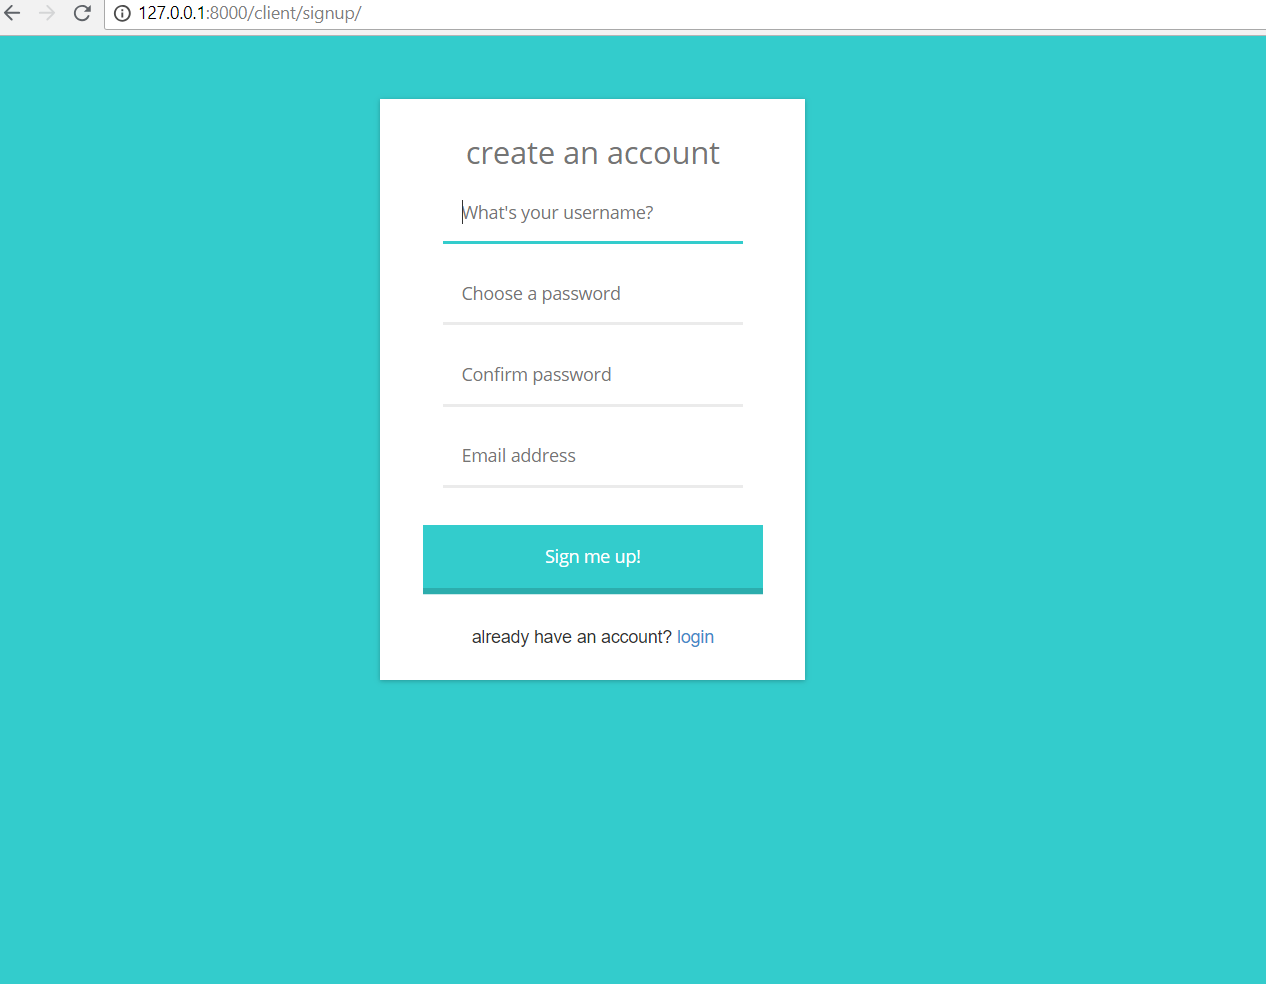
\includegraphics[scale=0.295]{sign_up.PNG}
    \caption{Signup page}
    \label{fig:Signup page}
\end{figure}

\begin{figure}[h]
    \centering
    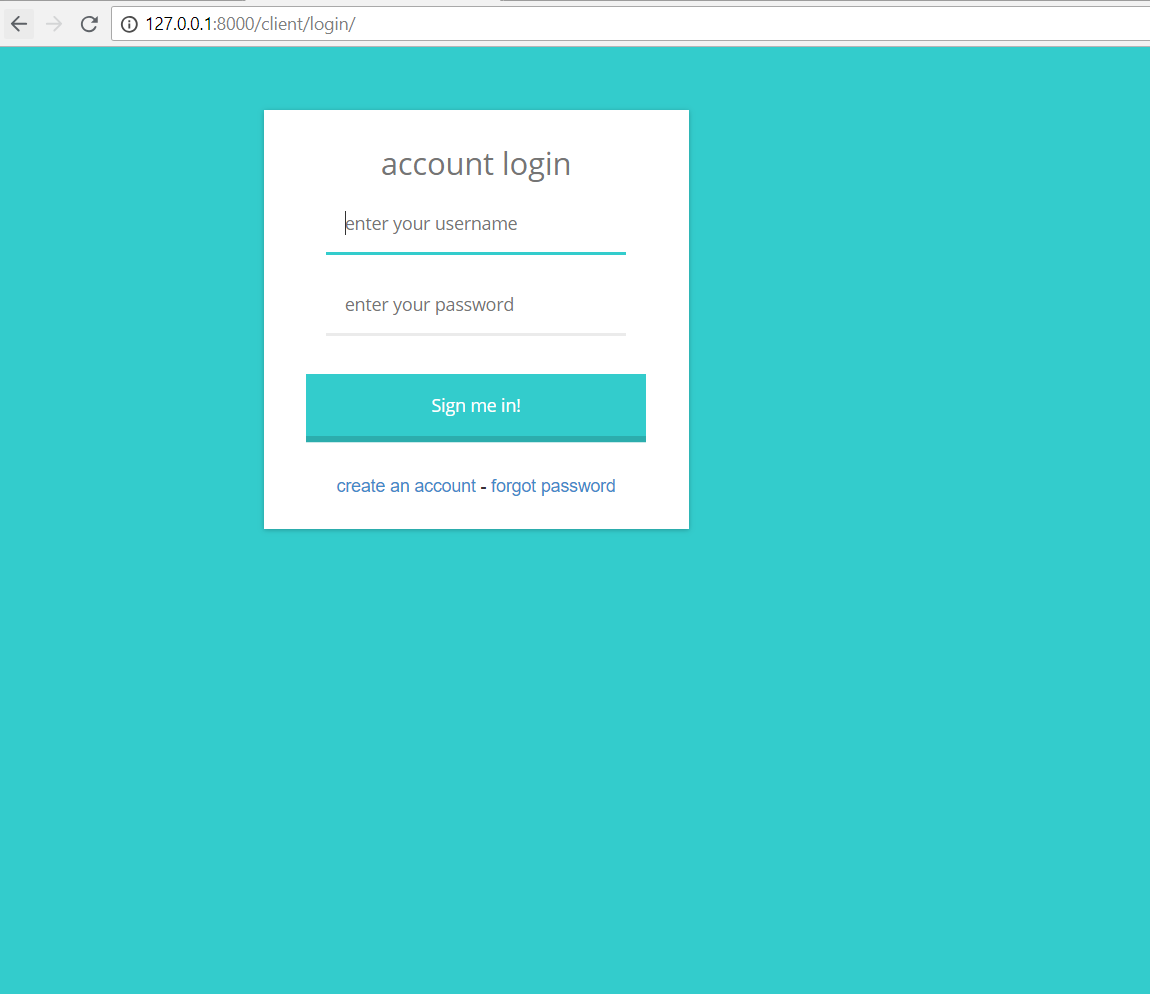
\includegraphics[scale=0.295]{log_in.PNG}
    \caption{Login page}
    \label{fig:Login page}
\end{figure}

\begin{figure}[h]
    \centering
    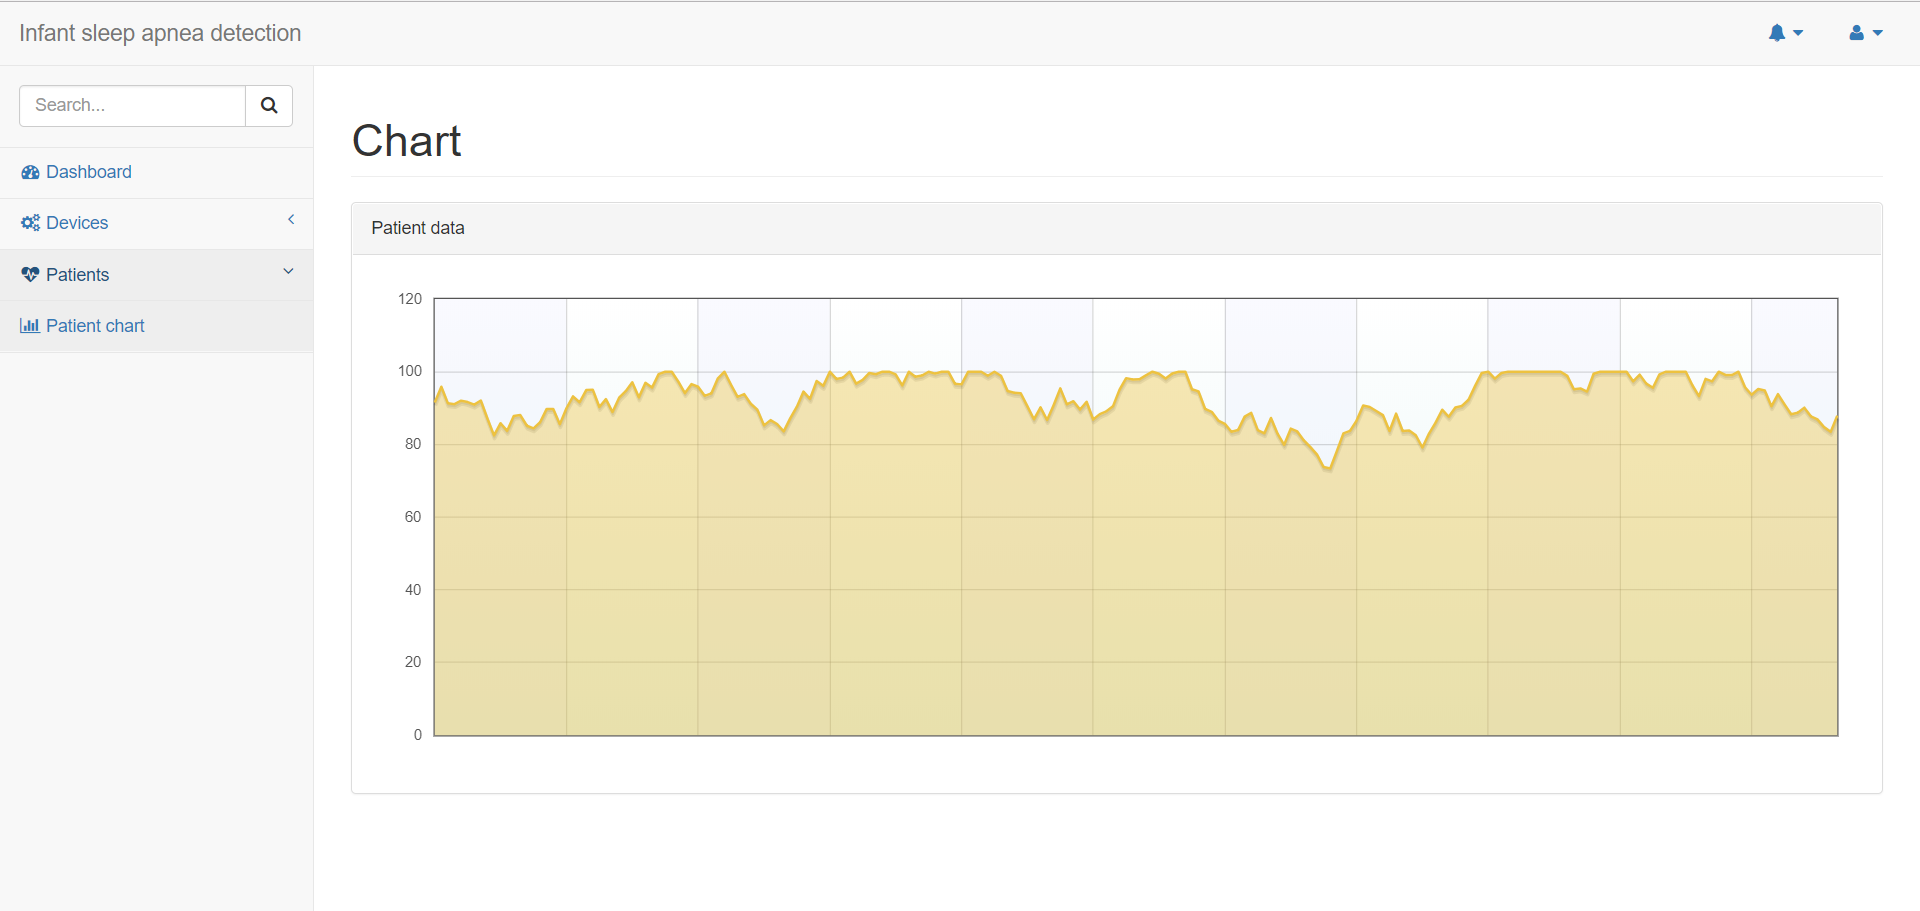
\includegraphics[scale=0.3]{chart.png}
    \caption{Breathing pattern reports}
    \label{fig:Breating pattern reports}
\end{figure}


\begin{figure}[h]
    \centering
    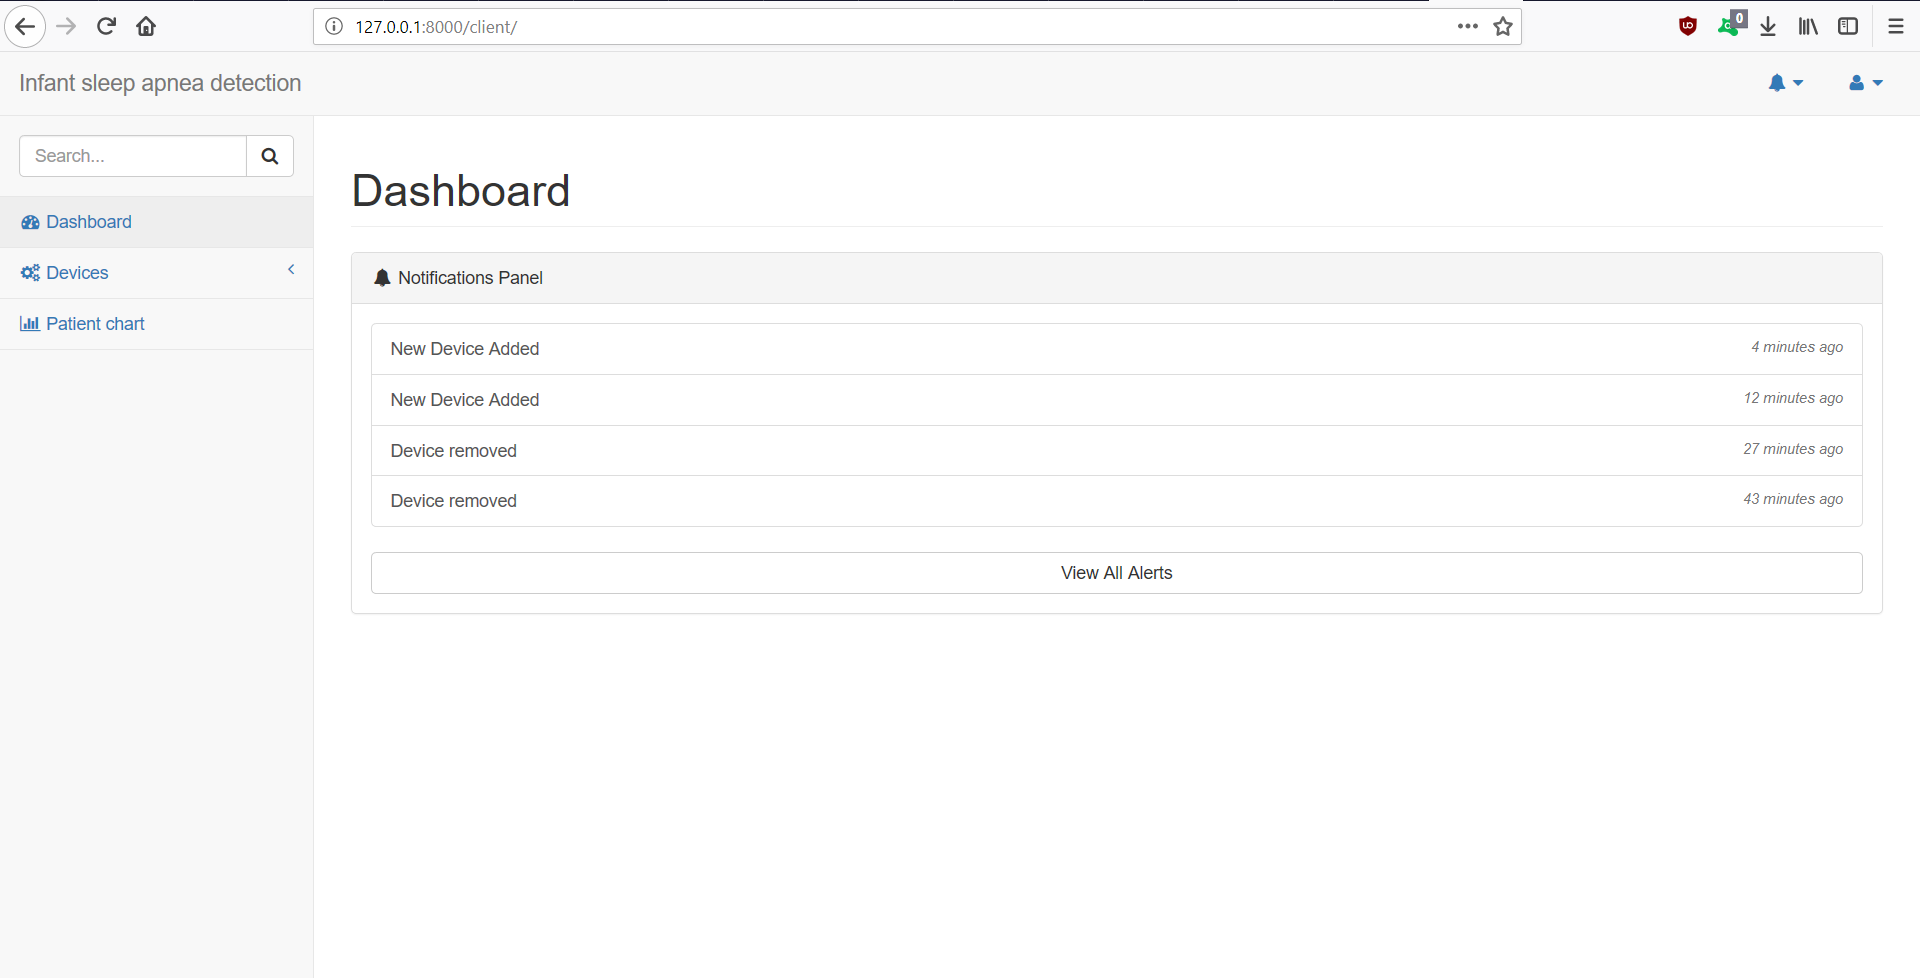
\includegraphics[scale=0.3]{dashboard.png}
    \caption{Notifications}
    \label{fig:Notifications}
\end{figure}

\begin{figure}[h]
    \centering
    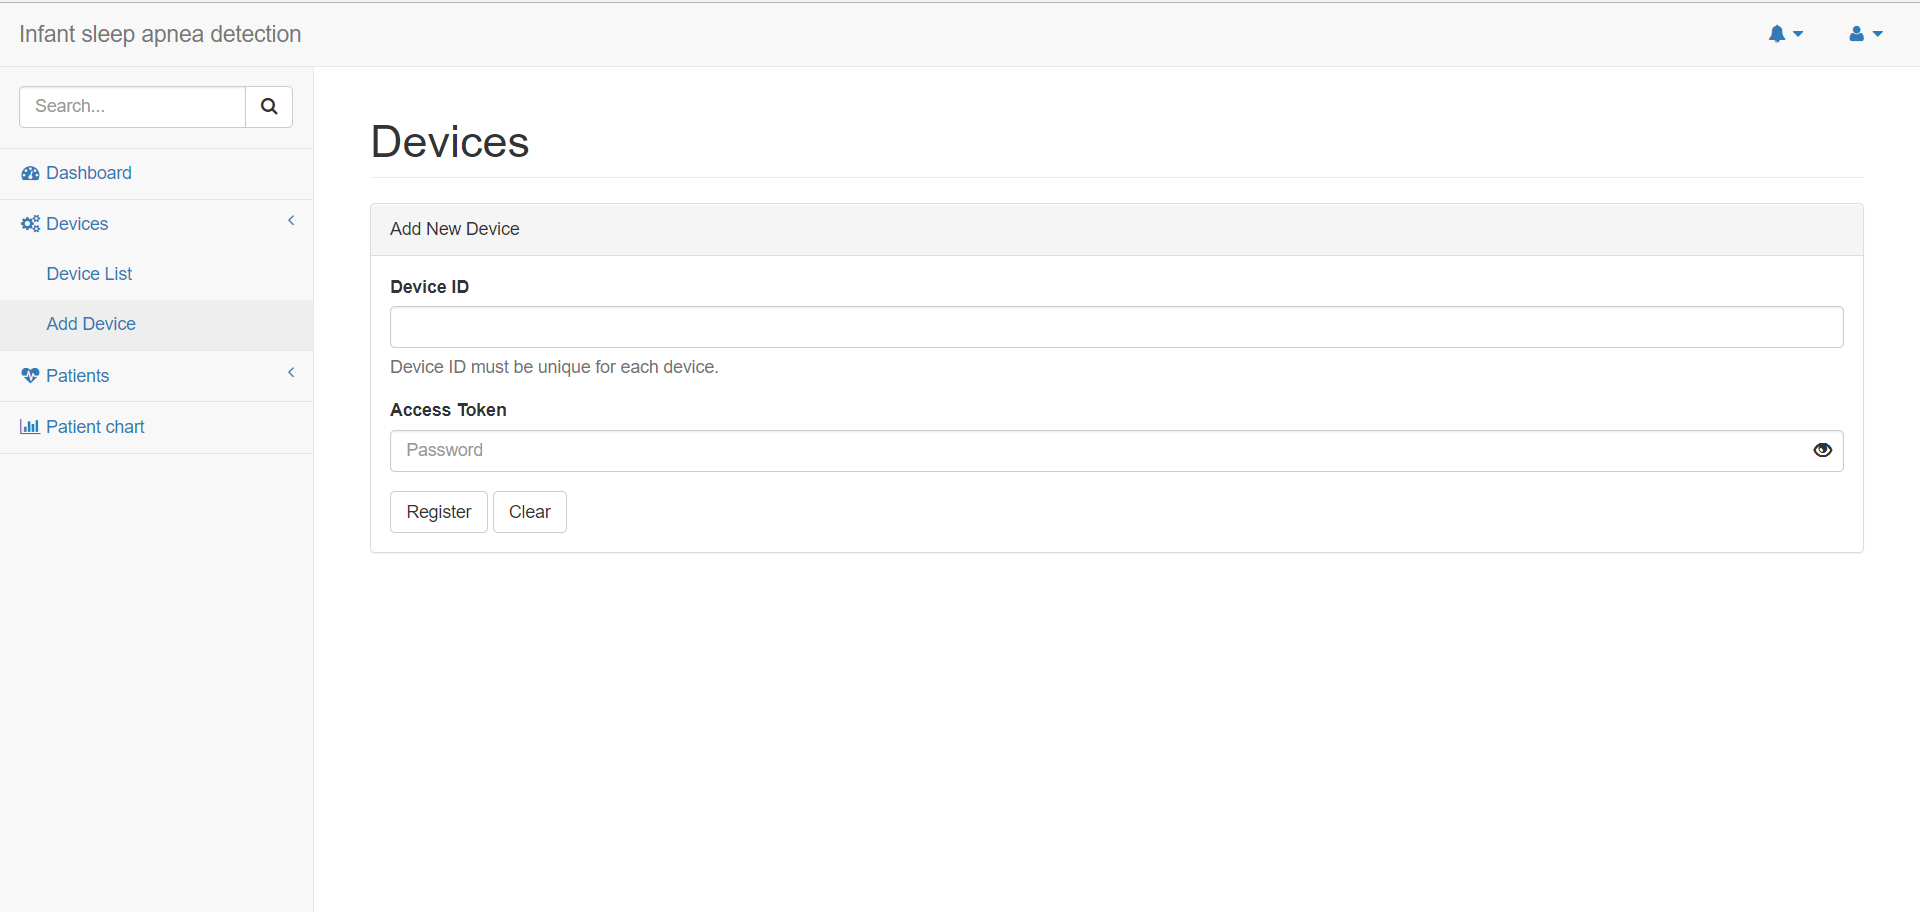
\includegraphics[scale=0.3]{adddevice.png}
    \caption{Add device}
    \label{fig:Add device}
\end{figure}

\begin{figure}[h]
    \centering
    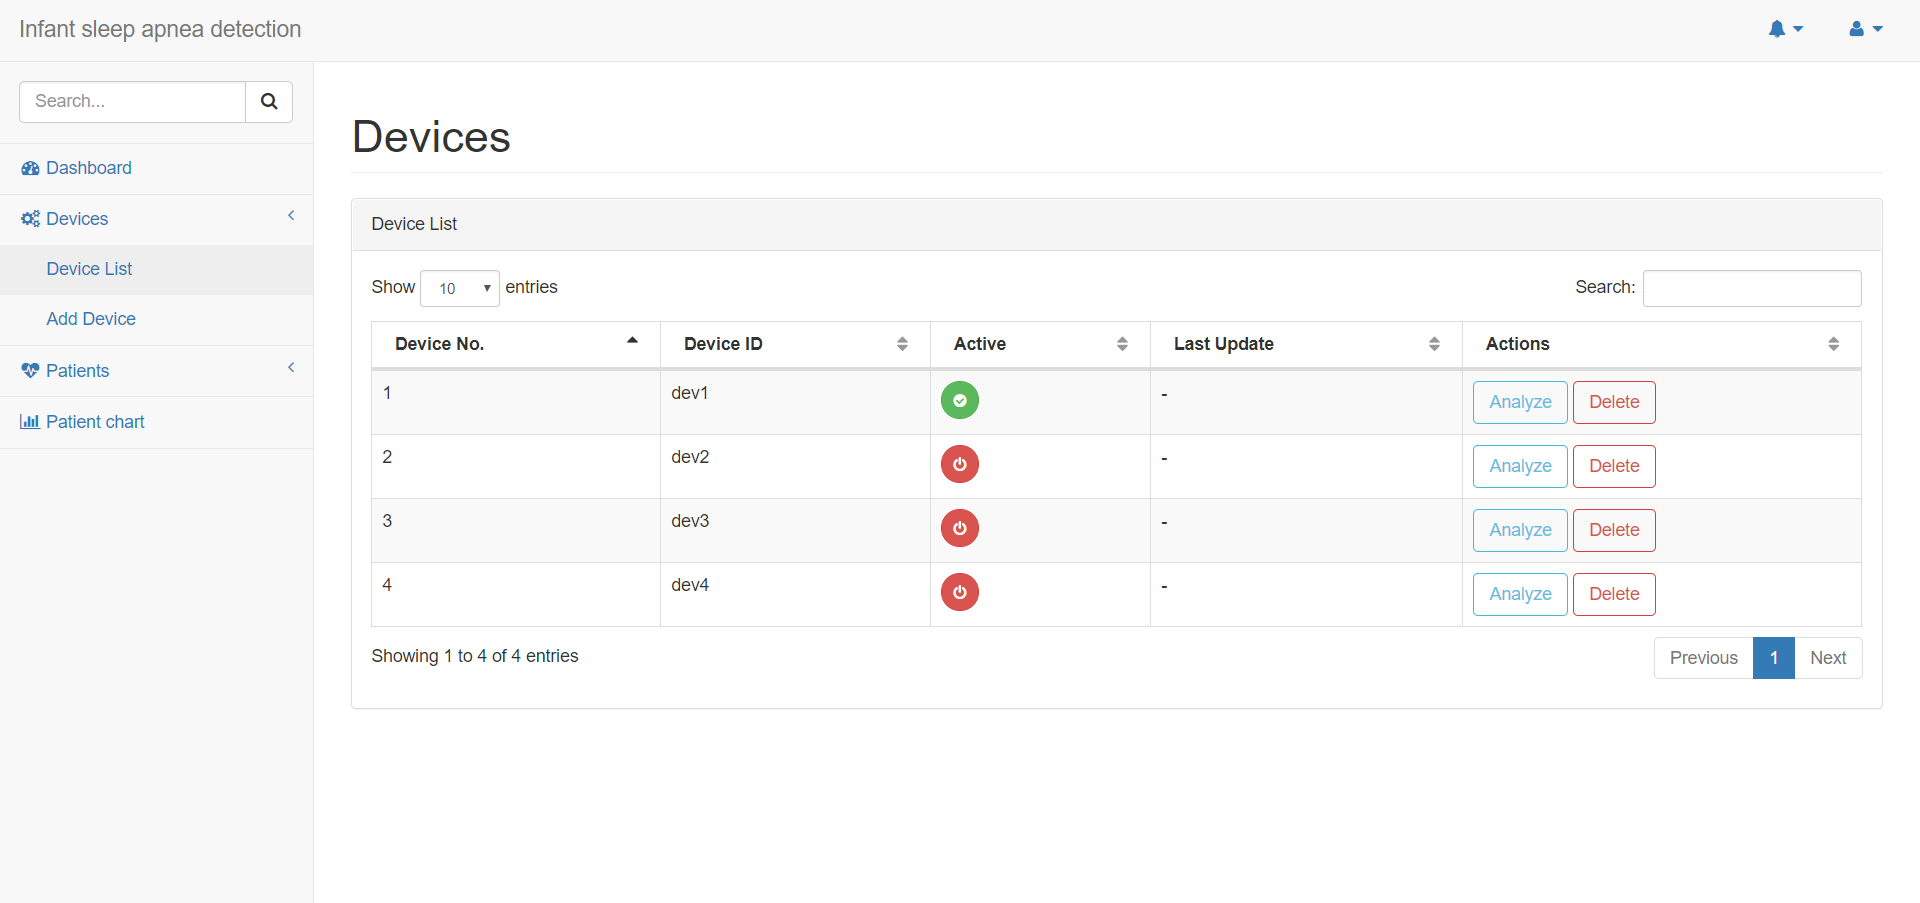
\includegraphics[scale=0.3]{listdevice.png}
    \caption{List of devices}
    \label{fig:List of devices}
\end{figure}

\begin{figure}[h]
    \centering
    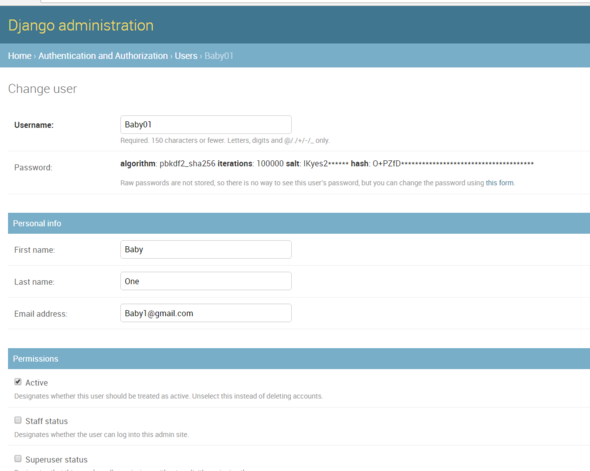
\includegraphics{deviceAdmin.png}
    \caption{Device administration}
    \label{fig:Device administration}
\end{figure}
\clearpage
\LARGE \centering END

\end{document}

